%!TEX root = ../ENTRUST_TR.tex

\begin{figure}
\centering
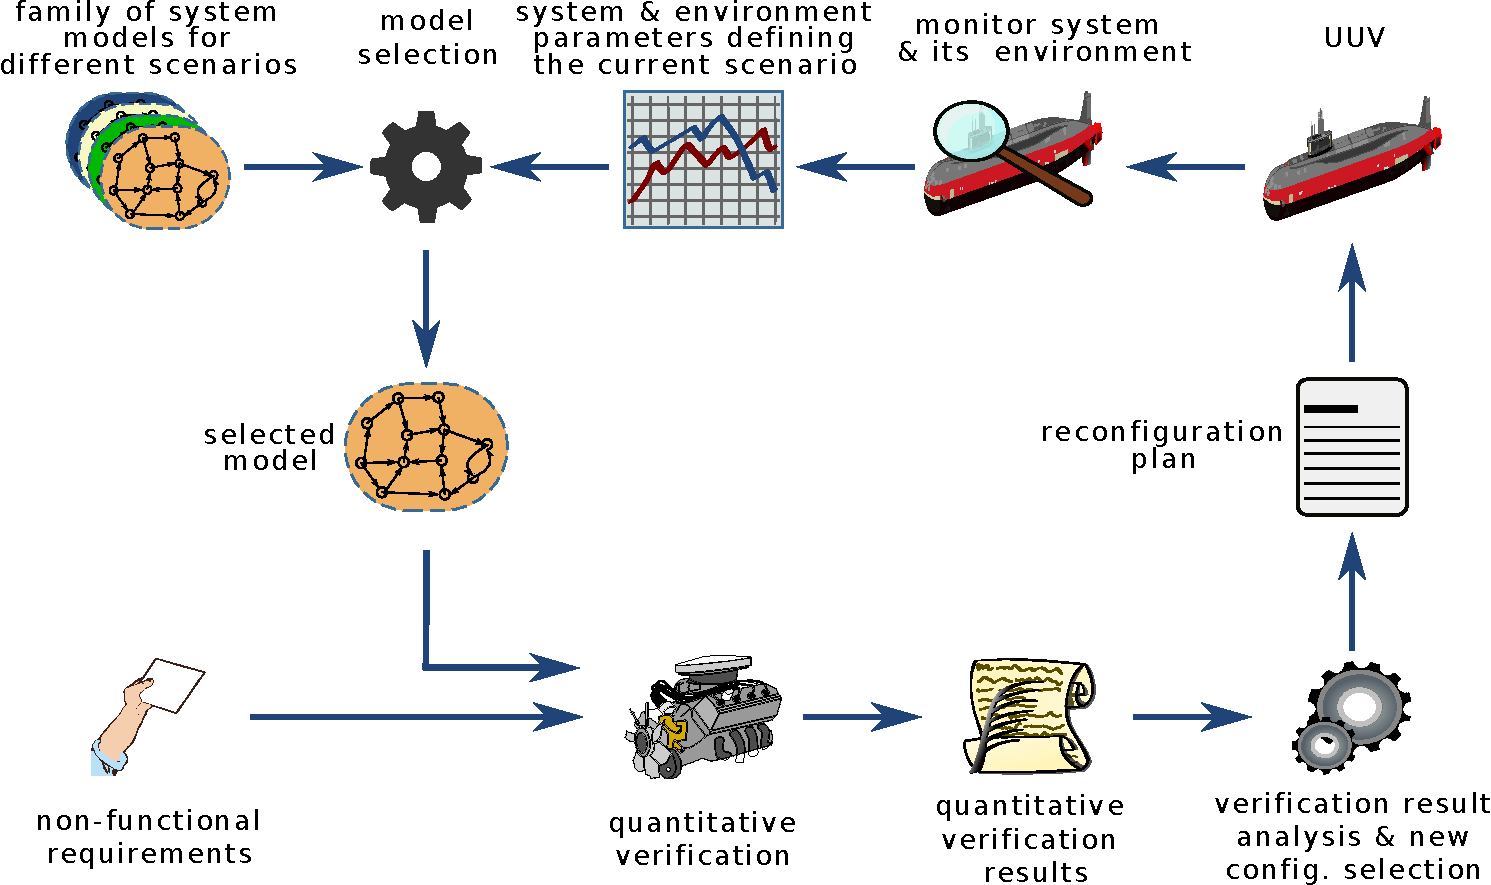
\includegraphics[width=0.75\hsize]{figures/rqv.pdf}
\caption{RQV-based self-adaptive system}
\label{fig:RQV}

\vspace*{-2mm}
\end{figure}

\textit{Runtime quantitative verification} (RQV) \cite{Calinescu2012:CACM} is an approach to implementing the closed control loop of self-adaptive systems in which the adaptation decisions are driven by the continual verification of stochastic models. RQV was introduced in~\cite{Calinescu2009:ICSE,Epifani2009:ICSE}, refined further in~\cite{Calinescu2011:TSE,Filieri2011:ICSE,Johnson2013:CBSE} and applied successfully in multiple application domains including dynamic power management~\cite{Calinescu2009:ICSE}, reconfiguration of data-centre infrastructure~\cite{Johnson2013:CBSE}, management of telehealth service-based system~\cite{Calinescu2011:TSE}, and self-optimising unmanned underwater vehicles~\cite{Gerasimou2014:SEAMS}.


Figure~\ref{fig:RQV} depicts the adaptation workflow of an RQV-based self-adaptive system. The approach involves monitoring the system (e.g., the UUV) and its environment continuously, to discover relevant changes and quantify them using fast on-line learning techniques. When these changes are significant and/or periodically, an RQV step is triggered, to identify which scenario the system operates in, and to select the associated model from a family of system models (i.e., a \emph{parametric model}) that correspond to different such scenarios. The selected model is then analysed using quantitative verification, to identify and/or predict violations of QoS requirements such as response time, availability and cost. When QoS violations are identified or predicted, the verification results support the selection of a new set of values for the configurable system parameters, so that enforcing this new configuration is \emph{guaranteed} to restore or maintain compliance with QoS requirements, respectively.

\begin{example}
Figure~\ref{fig:model} depicts the CTMC model $M_i$ of the $i$-th sensor of the UUV from our running example. The CTMC starts in state 0 and transitions in state 1 if the sensor is switched on ($x_i=1$) or in state 6 otherwise ($x_i=0$). With rate $r_i$,  a measurement is performed, as indicated by the transition between states 1 and 2. The measurement is ``sufficiently accurate" with probability $p_i$ and the transition between states 2 and 3 is taken, whereas the transition between states 2 and 4 is enabled in case of an inaccurate measurement. An active sensor continues taking measurements while it is active,  as modelled by the transition between states 5 and 1. The CTMC model is augmented with two cost/reward structures, whose non-zero elements are shown in Fig.~1 in rectangular boxes, and dashed rectangular boxes, respectively. The former, ``\textit{energy}'' structure associates the energy used to switch the sensor on (i.e., $e_i^\mathrm{on}$) and off (i.e., $e_i^\mathrm{off}$) and to perform a measurement (i.e., $e_i$) with the CTMC transitions that model these events. Note that the ternary expression ``$\mathit{condition}?a\!:\!b$'' was used to indicate that the energy $e_i^\mathrm{on}$ is consumed only if the previous state of the sensor was ``off'', i.e., if $x_i^\mathrm{old}=0$, whereas the energy $e_i^\mathrm{off}$ is used  only if the opposite is true ($x_i^\mathrm{old}=1$). As concerns the latter, ``\textit{measurement}'' cost/reward structure, it associates a reward of $1$ with the transition that corresponds to an accurate measurement. 
\end{example}

\begin{figure}[t]
\centering 
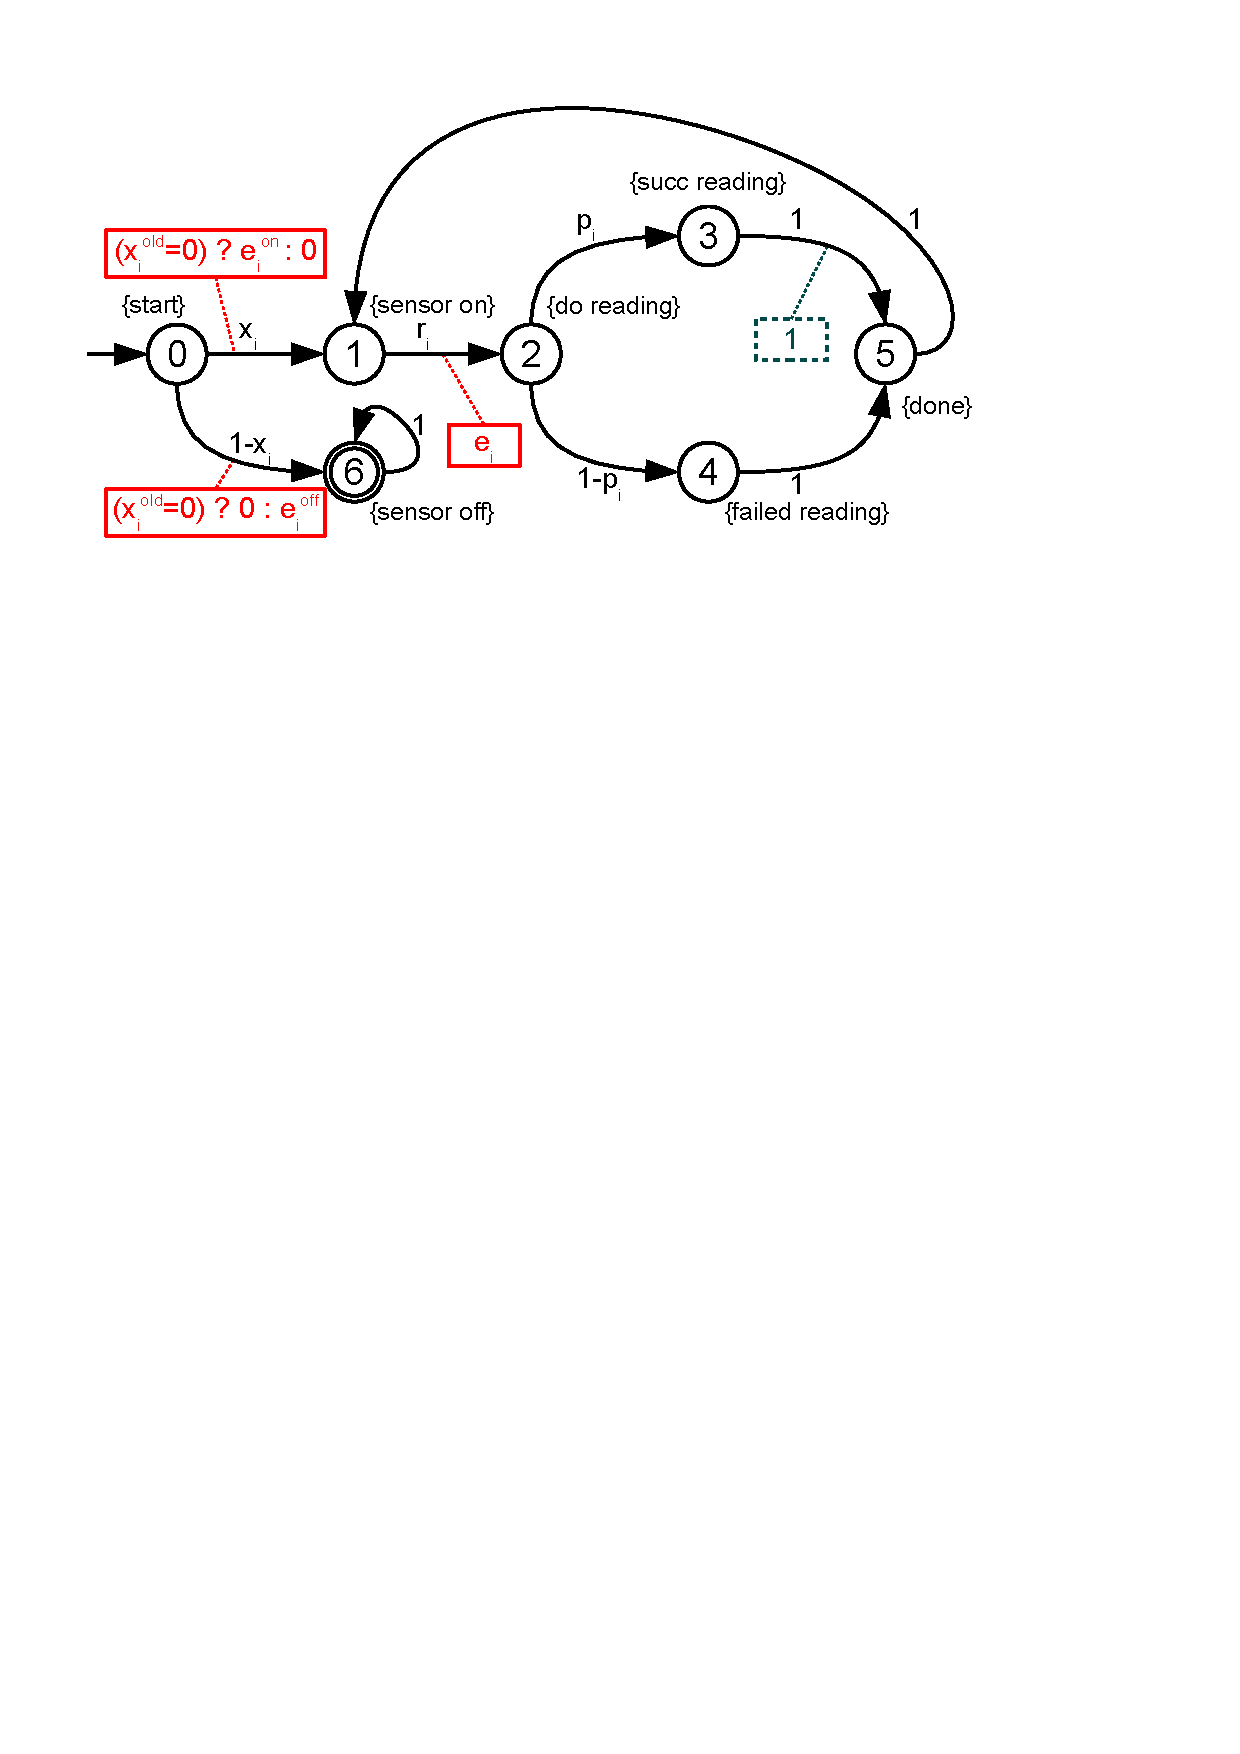
\includegraphics[trim = 17mm 205mm 45mm 17mm, clip, width=0.7\linewidth]{figures/model.pdf}
\caption{CTMC model $M_i$ of the $i$-th UUV sensor}
\label{fig:model}

\vspace*{-2mm}
\end{figure}